\documentclass[11pt]{article}

\usepackage[letterpaper,margin=0.75in]{geometry}
\usepackage{booktabs}
\usepackage{graphicx}
\usepackage{listings}

\setlength{\parindent}{1.4em}

\newcommand{\code}[1]{\texttt{#1}}

\begin{document}

\lstset{
  language=Python,
  basicstyle=\small,          % print whole listing small
  keywordstyle=\bfseries,
  identifierstyle=,           % nothing happens
  commentstyle=,              % white comments
  stringstyle=\ttfamily,      % typewriter type for strings
  showstringspaces=false,     % no special string spaces
  numbers=left,
  numberstyle=\tiny,
  numbersep=5pt,
  frame=tb,
}

\title{Lab 3 Report}

\author{Nate Fox}

\date{}

\maketitle

\section{Congestion Control}

\subsection{Class Variables}
To implement congestion control, I started by changing some of the TCP class variables. I renamed the \code{window} variable to \code{cwnd} in order to match the variable names from the textbook, and I initialized \code{cwnd} to be one MSS. I also introduced the \code{ssthresh} variable to keep track of the slow start threshold. Finally I introduced the \code{ack\_count} variable to keep track of duplicate ACKs.

\subsection{Receiving New ACKs}
When I receive ACKs for newly acknowledged data, I update my congestion window according to what state I am in. If my current \code{cwnd} is less than \code{ssthresh}, I consider myself in slow start mode and I increment \code{cwnd} by the number of new bytes acknowledged. If my current \code{cwnd} is greater than or equal to \code{ssthresh}, I consider myself in AIMD mode and I increment \code{cwnd} by (MSS * new\_bytes / \code{cwnd}). I also reset my \code{ack\_count} to 0.
 
\subsection{Receiving Duplicate ACKs}
When I receive a duplicate ACK, I increment my \code{ack\_count}. If \code{ack\_count} is three after I increment it, I retransmit without restarting the retransmission timer or updating the RTO.

\subsection{Retransmitting}
Whenever I retransmit, either due to the retransmission timer firing or due to three duplicate ACKs, I update the \code{ssthresh} and the \code{cwnd}. I set \code{ssthresh} to one-half of \code{cwnd} (to a minimum of one MSS) and I reset \code{cwnd} to one MSS.

\pagebreak
\section{Tests}

\subsection{Slow Start}
To test the slow start mode, I set the queue size on the link to 100 packets and I set the \code{ssthresh} to 100,000 bytes. I transfer a small 64 kb file, which is guaranteed to not overwhelm the queue.

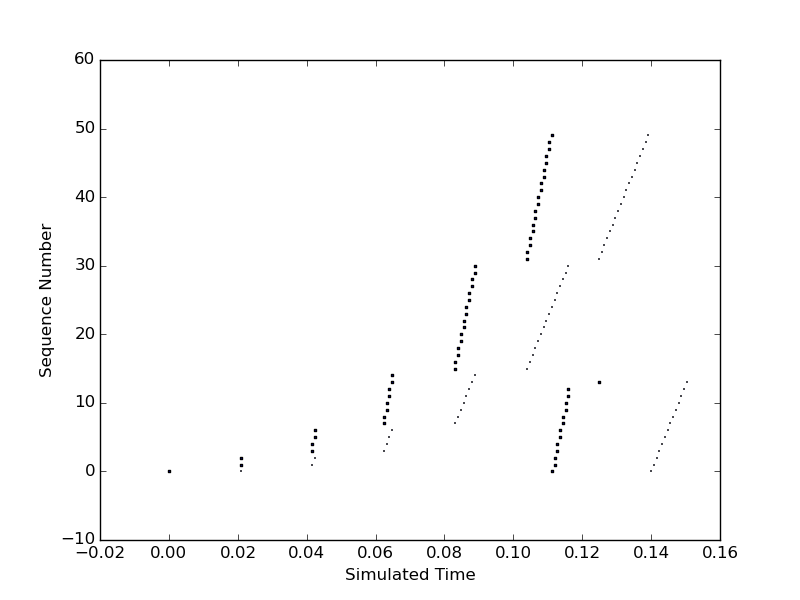
\includegraphics[width=10cm]{../graphs/slow_start.png}

The above graph shows that \code{cwnd} starts at one MSS, then doubles each round. When the \code{cwnd} size is 64,000 bytes, there are only 1000 bytes left to send, which is why the final round shows only a single packet.

\subsection{Additive Increase}
To test additive increase mode, I set the queue size on the link to 100 packets and I set the \code{sstrhesh} to 16,000 bytes. I transfer a small 64 kb file, which is guaranteed to not overwhelm the queue.

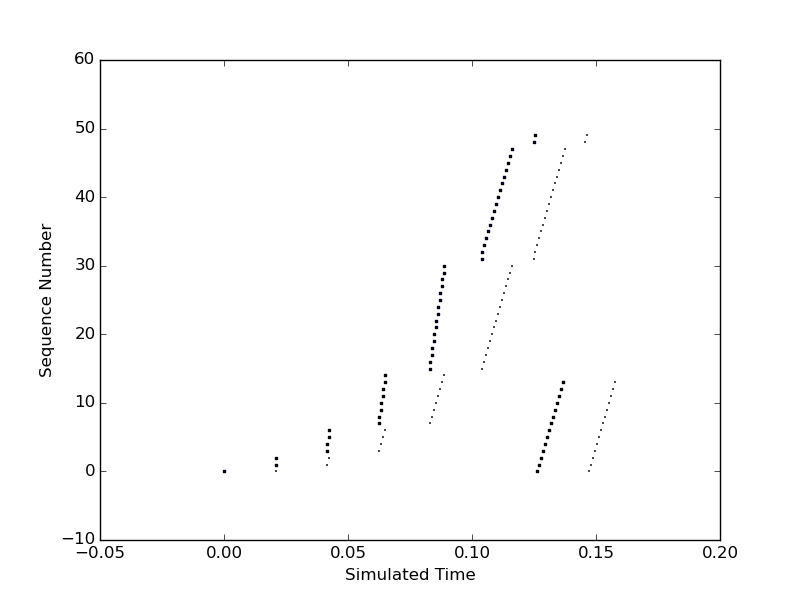
\includegraphics[width=10cm]{../graphs/additive_increase.png}

The above graph shows that \code{cwnd} starts at one MSS, then doubles each round until \code{cwnd} is 16,000 bytes. Once it hits the 16,000 byte threshold, it goes into additive increase mode. It sends 17 packets for the following round.

\pagebreak
\subsection{AIMD}
To test AIMD, I reset the \code{ssthresh} to 100,000 and I set the queue size on the link to 15 packets, which causes a packet to be dropped once \code{cwnd} grows to 32,000 bytes. I transfer a 512 kb file.

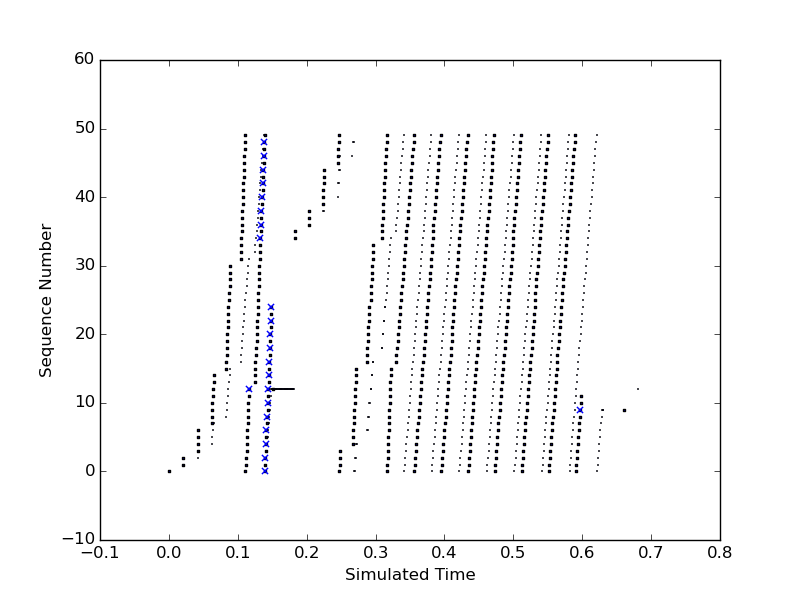
\includegraphics[width=10cm]{../graphs/aimd_with_mod.png}

The above graph shows that \code{cwnd} starts at one MSS, then doubles each round until \code{cwnd} is 64,000 bytes. The last packet sent when \code{cwnd} is 32,000 bytes gets dropped, but the sender has not yet received the three duplicate ACKs, so it continues in slow start mode, which leads to multiple other packets getting dropped. Once the three duplicate ACKs are received, the sender resets \code{cwnd} to one MSS and goes back into slow start mode, but now with \code{ssthresh} set to 32,000 bytes. Once \code{cwnd} gets up to 32,000 bytes in slow start mode, it goes into AIMD mode. Below is the same graph without the modulo sequence numbers for added clarity:

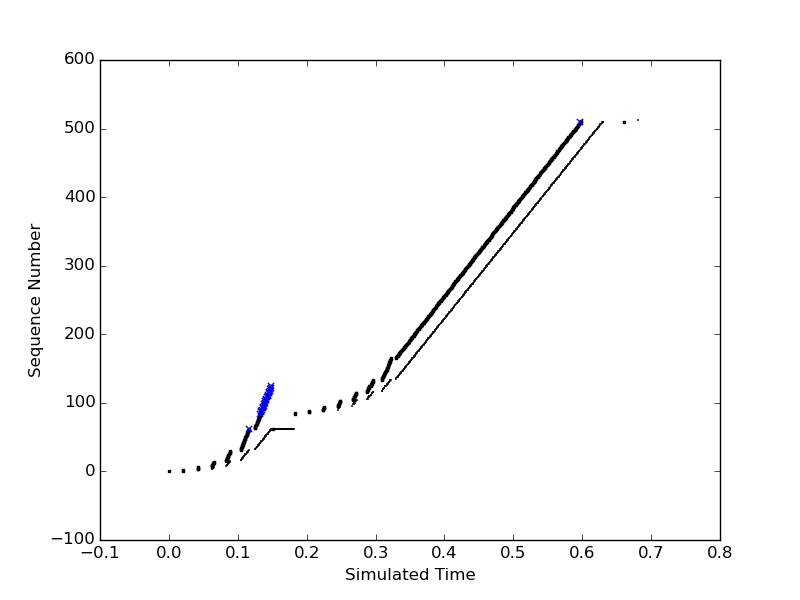
\includegraphics[width=10cm]{../graphs/aimd_no_mod.png}

\pagebreak
\subsection{Burst Loss}
To test the response to multiple packets being lost at once, I keep the \code{ssthresh} at 100,000 and I set the queue size on the link to 10 packets. I transfer a 256 kb file.

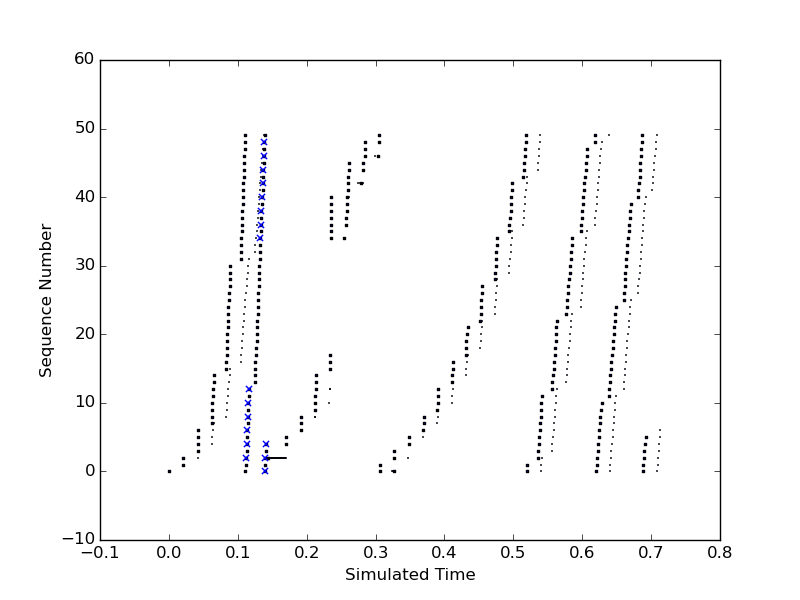
\includegraphics[width=10cm]{../graphs/burst_loss_with_mod.png}

The above graph shows that multiple packets are dropped when the \code{cwnd} is at 32,000 bytes. The sender gets three duplicate ACKs for ACK values 52000, 84000, 92000, 96000, and 100000. This causes the \code{ssthresh} to drop from 100,000 bytes to 1,000 bytes over a 0.3-second period. Once the sender receives the ACK for 102,000, the sender is in a constant state of additive increase. Below is the same graph without the modulo sequence numbers for added clarity:

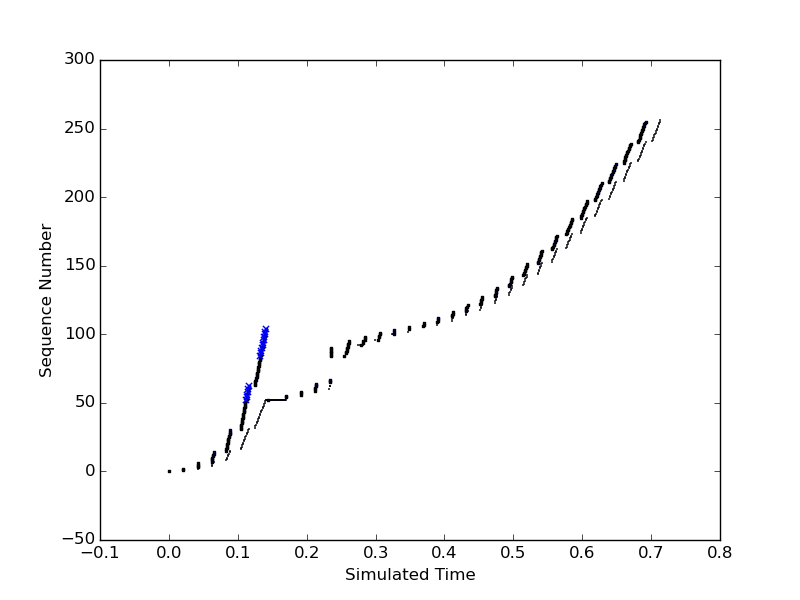
\includegraphics[width=10cm]{../graphs/burst_loss_no_mod.png}

\end{document}
